\scanpage{118}
\diagram{\begin{tikzcd}[ampersand replacement=\&,execute at end picture={
 \begin{scope}[x=.012cm,y=-.012cm,every node/.style={font=\scriptsize,inner sep=.5pt}]
 \coordinate (u) at (327,380); \coordinate (v) at (497,387); \coordinate (w) at (410,265);
 \draw (u)--(w)--(v)--cycle;
 \node[below right] at (u) {$u$};\node[below left] at (v) {$v$};\node[right] at (w) {$w$};
 \draw (u)--(87,314)--(79,354)--cycle (u)--(86,394)--(95,437)--cycle
       (u)--(145,501)--(166,532)--cycle (u)--(217,549)--(258,567)--cycle;
 \draw (v)--(679,311)--(677,352)--cycle (v)--(667,420)--(657,447)--cycle
       (v)--(657,504)--(635,528)--cycle (v)--(549,549)--(520,560)--cycle;
 \draw (w)--(264,168)--(290,133)--cycle (w)--(329,120)--(347,100)--cycle
       (w)--(409,100)--(445,101)--cycle (w)--(554,131)--(574,151)--cycle;
 \node[left] at (81,310) {$\alpha'_4$};\node[left] at (78,353) {$\alpha_4$};
 \node[left] at (89,391) {$\alpha'_3$};\node[left] at (94,435) {$\alpha_3$};
 \node[left] at (145,498) {$\alpha'_{\unsure{2}}$};\node[below] at (159,532) {$\alpha_2$};
 \node[left] at (217,553) {$\alpha'_1$};\node[right] at (252,570) {$\alpha_1$};
 \node at (36,332) {$a_4\big\{$};\node at (39,422) {$a_3\big\{$};
 \node at (91,551) {$a_2\big\{$};\node[below] at (218,584) {$\underbrace{\hspace{2em}}_{a_1}$};
 \node[right] at (677,311) {$\beta_1$};\node[right] at (677,347) {$\beta'_1$};
 \node[right] at (667,416) {$\beta_2$};\node[right] at (657,444) {$\beta'_2$};
 \node at (756,335) {$\big\}b_1$};\node at (770,439) {$\big\}b_2$};\node at (720,548) {$\big\}b_3$};
 \node[below] at (511,560) {$\unsure{\beta'_4|\beta'_3}$};\node[right] at (546,551) {$\unsure{\beta_4|\beta_3}$};
 \node[below] at (572,589) {$\underbrace{\hspace{2em}}_{b_4}$};
 \node[left] at (265,167) {$\gamma_1$};\node[left] at (289,131) {$\gamma'_1$};
 \node[above] at (324,121) {$\gamma_2$};\node[above] at (351,100) {$\gamma'_2$};
 \node[above] at (407,99) {$\gamma_3$};\node[above] at (455,102) {$\gamma'_3$};
 \node[above] at (556,129) {$\deleted{\unsure{\alpha}}\gamma_4$};
 \node[right] at (574,154) {$\gamma'_4$};
 \node[rotate=45] at (194,123) {$c_1\big\{$};
 \node at (337,44) {$\overbrace{\hspace{2em}}^{c_2}$};
 \node at (443,29) {$\overbrace{\hspace{2em}}^{c_3}$};\node at (681,94) {$\big\}c_4$};
 \draw[thin] (128,66)--(278,230)--(505,579);
 \end{scope}}]\phantom{.}\end{tikzcd}}
\[
 12\ \text{arêtes}\ \left\{\begin{array}{lll}
 \alpha_1,\alpha_2,\alpha_3,\alpha_4&\text{\unsure{liés|liées} à}&\beta_4\\
 \beta_1,\beta_2,\beta_3,\beta_4&\text{-------}&\gamma_4\\
 \gamma_1,\gamma_2,\gamma_3,\gamma_4&\text{-------}&\alpha_4
 \end{array}\right.
\]
\[
 \deleted{12\ \text{arêtes}\ \left\{\begin{array}{lll}
 \alpha_i&\text{lié à}&\alpha'_i\\\beta_i&\text{lié à}&\beta'_i\\\gamma_i&\text{lié à}&\gamma'_i
 \end{array}\right.\quad 1\le i\le\unsure{4|7}}
\]
\[
 12\left\{\begin{array}{ll}
 \alpha'_i\ \text{liés à}&\beta'_4\\ \beta'_i\ \text{------}&\gamma'_4\\ \gamma'_i\ \text{------}&\alpha'_4
 \end{array}\right.
\]
% margin note written sideways
\margin{\(a_1\wedge\underbrace{\unsure{x_2|a_2}\wedge\unsure{x_3|a_3}}=1\)}
\[
 \left\{\begin{array}{lll}
 \alpha_1&\text{lié à}&\beta'_1,\beta_2,\beta_3,\beta_4\\
 \alpha_2&\text{------}&\beta_1,\beta'_2,\beta_3,\beta_4\\
 \alpha_3&\text{------}&\beta_1,\beta_2,\beta'_3,\beta_4\\
 \alpha_4&\text{------}&\beta'_1,\beta'_2,\beta'_3,\beta_4
 \end{array}\right.
 \quad
 \begin{gathered}\alpha'_1\ \text{lié à}\ \beta_1,\beta'_2,\beta'_3,\beta'_4\\\text{----}\end{gathered}
\]
% margin note written sideways
\margin{\({}_{G_2}P_1\underset{G_3}{\wedge}(\unsure{U}P_2\underset{G_3}{\wedge}P_3)_{G_2}\)}
\[
 \boxed{\begin{aligned}\alpha_1&\text{ lié à }\beta'_1\\ \alpha_{\unsure{1|2}}&\text{ lié à }\beta_2\end{aligned}}
 \quad\underset{\longleftarrow}{\boxed{\alpha_1\text{ lié à }\gamma'_4}}
 \quad
 \begin{aligned}
 \alpha_{\unsure{3|1}}&\text{ lié à }\deleted{\unsure{\gamma}}\beta_4\text{ et }\gamma'_4\\
 \beta_1&\text{ lié à }\gamma_4\text{ et }\beta'_4\\
 (\alpha_1&\text{ lié à }\beta_1)\Rightarrow\\
 \alpha_1&\text{lié}
 \end{aligned}
\]
\diagram{\begin{tikzcd}[ampersand replacement=\&,row sep=.8em,column sep=.6em]
 \&\&w\&\&\\
 \&u\arrow[ur]\arrow[rr,dash]\arrow[dl,dash]\arrow[d,dash]\&\&v\arrow[ul,dash]\arrow[d,dash]\arrow[dr,dash]\arrow[drr,dash]\&\&\\
 \unsure{\alpha|v}\&\unsure{\alpha'|\alpha_2}\&\&\beta\&\beta'\&\beta''\\
 {\Vert}\&{\Vert}\&\&{\Vert}\&{\Vert}\&\\
 \unsure{\alpha_1|\alpha}\&\alpha'_2\&\&\beta'_1\&\beta_2\&
\end{tikzcd}}
\[
 \left\{\begin{array}{lll}
 \alpha_1&\beta'_1,&\gamma'_4\\\alpha_1,&\beta_2,&\gamma_{\unsure{2|3}}\\
 \alpha'_2,&\beta'_1,&\gamma'_3\\\alpha'_2,&\beta_2,&\gamma_4
 \end{array}\right.
\]
% margin note written sideways; group calculations run upwards from the right edge.
\[
\begin{aligned}
 &\deleted{g_2a_1g_3^{-1}=1}\\
 &g_2(\alpha_2a_1\alpha_3^{-1})g_3^{-1}=\alpha_2a_1\alpha_3\\
 &(g_2\alpha_2)a_1(\deleted{\unsure{\alpha}}g_3\alpha_3)^{-1}=\alpha_2a_1\alpha_3\\
 &g_3\alpha_3=\widetilde a_1(g_2\alpha_2)\\
 &\widetilde a_1(g_2)\widetilde a_1(\alpha_2)\unsure{'|,}=g_3\alpha_3\\
 &g_3=\\
 &\widetilde A_1(g_2)\alpha_3=\widetilde a_1(g_2)\deleted{\unsure{\alpha}}\widetilde a_1(\alpha_2)\\
 &\widetilde A_1(g_2)=\widetilde a_1(g_2)\widetilde a_1(\alpha_2)\alpha_3^{-1}
\end{aligned}
\]
\figure{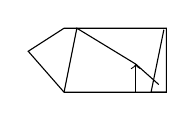
\begin{tikzpicture}[x=.65cm,y=.65cm]
 \draw (0,0)--(-.7,.8)--(0,1.25)--(2,1.25)--(2,0)--cycle;
 \draw (0,0)--(.25,1.25)--(1.4,.55)--(1.85,.15);
 \draw[->] (1.4,0)--(1.4,.55);
 \draw (1.7,0)--(1.95,1.22) (1.7,0)--(2,0);
\end{tikzpicture}}
% Lower-edge text is inverted relative to the large graph.
\[
\begin{aligned}
 &g_2a_1=a_1g_3\deleted{=b_1}&&\text{i.e. }g_2a_1g_3^{-1}=a_1\\
 &g_3a_2=a_2g_1=b_2&&\text{i.e. }g_3a_2g_1^{-1}=a_2\\
 ?\ \Downarrow\quad&g_1a_3=a_3g_2&&a_1,a_2,
\end{aligned}
\]
\[
 \underbrace{(g_1,g_2,g_3)\underbrace{(a_1,a_2,a_3)}_{\in \Gamma}}_{\in \Gamma}
       =(a_1,a_2,\unsure{a_3|a'_3})
\]
% archive sheet number: 119
